\documentclass[../thesis.tex]{subfiles}

\begin{document}

\chapter{Conclusion}
\label{chap:conclusion}

\section{Relevance of $\theta_{13}$ to future research}
\label{sec:futureRelevance}

Quantitatively, the value of $\theta_{13}$ is broadly useful in the context of beyond-the-Standard-Model (BSM) model building. More concretely, however, $\theta_{13}$ is important in the context of unraveling two extremely significant properties of neutrinos: The value of $\dcp$, and the mass hierarchy (MH). In this context, the importance of $\theta_{13}$ arises simply from the fact that $\dcp$ and the MH both influence oscillation probabilities via higher-order terms that are controlled by e.g. \(\sin^2\theta_{13}\) or \(\sin^2 2\theta_{13}\); thus, a larger $\theta_{13}$ (up to a certain point) implies a greater experimental sensitivity to these subtle effects. In turn, $\dcp$ and the MH are pivotal in relation to two of the biggest questions in particle physics: The origin of the the matter-antimatter asymmetry of the Universe, and the Majorana nature (or lack thereof) of the neutrino, respectively.

\subsection{Baryon asymmetry and $\dcp$}
\label{sec:baryonAsym}

Most physical processes produce, in aggregate, equal amounts of matter and antimatter. And yet, our present universe contains a clear excess of matter. The origin of this excess thus demands our investigation. Although the specific mechanisms at play remain unknown, together they must fulfill the \emph{Sakharov conditions.} As most of the normal matter in the Universe is baryonic, explaining the matter-antimatter asymmetry largely boils down to explaining \emph{baryogenesis,} the generation of excess baryons over antibaryons. The three Sakharov conditions, in the context of baryogensis, are:

\begin{enumerate}
\item Existence of processes that violate baryon number symmetry $B$; otherwise, every baryon would be created in concert with an antibaryon
\item Existence of processes that violate C and CP symmetry; otherwise the C and CP-conjugates of $B$-violating interactions would cancel out the asymmetry
\item Lack of thermal equilibrium (at some point in history); otherwise, every process would be counterbalanced by its CPT-conjugate
\end{enumerate}

Within the SM, an asymmetry can theoretically be produced via the mechanism of electroweak baryogenesis. However, the only source of CP violation in the SM is the complex phase in the CKM matrix, and it is known that this effect alone is not large enough to account for the observed matter-antimatter asymmetry \cite{Shaposhnikov:2009zzc}. If the neutrino $\dcp$ is found to deviate significantly from zero (or $\pi$), then this would constitute a brand new source of CP violation, and if the effect is large enough, it could fully explain our matter-dominated universe (when harnessed by a BSM mechanism such as leptogenesis). Thus, $\dcp$, in a sense, could play a critical role in explaining why the universe is not a formless sea of photons. Conversely, if it is found to be small or consistent with zero, then the mystery of baryogenesis will be deepened even further. For these reasons, the measurement of $\dcp$ is a chief driving goal of some of the most ambitious neutrino oscillation experiments underway. This effort would be far more difficult if Nature had chosen a much smaller $\theta_{13}$.

\subsection{Majorana neutrinos and the mass hierarchy}
\label{sec:majorana}

As is illustrated in \autoref{fig:massOrdering}, the ordering of the neutrino masses is not fully known. Determining the mass hierarchy is an important effort in its own right. The MH affects cosmological models, kinematic measurements of the neutrino mass,
% (XXX is this true???),
the measurement of $\dcp$, and BSM model building, to name a few examples of its importance. It even relates to the question of the very nature of the neutrino mass, as we show here.

In the SM, the neutrino is a simple two-component left-handed \emph{Weyl} spinor. Once mass is added, however, the picture necessarily becomes more complicated. Massive spinors can be classified as either of Majorana or Dirac type. A Majorana spinor is, by definition, one that is invariant under the operation of charge conjugation (i.e., it is identical to its antiparticle). A Dirac spinor, on the other hand, is not self-conjugate, and contains twice as many components.

For a Majorana spinor, the Hamiltonian can contain a term (the Majorana mass) that contributes to the particle's mass and creates particle-particle pairs. Obviously, this is impossible if the particle carries any sort of conserved charge, as is the case for every particle of the SM, except (after electroweak symmetry breaking) the neutrino. Thus, the neutrino could prove to be the first known fundamental Majorana fermion, and if this is so, it would also provide the first example (via the Majorana mass) of lepton number violation.

The possible Majorana nature of the neutrino is closely related to the question of the smallness of the neutrino mass scale. Taking a step back, the simplest model of neutrino mass (which furnishes Dirac neutrinos) can be constructed in analogy with the masses of the other fermions: We introduce a sterile $\nu_{\text{R}}$ and construct a Yukawa coupling between it, the Higgs field, and the active $\nu_{\text{R}}$. The lack of a Majorana mass term means that $\nu_{\text{R}}$ and $\nu_{\text{L}}$ can be combined into a single Dirac spinor. Although this construction works, it suffers from the fact that the dimensionless coupling constant must be extremely small, of order $m_\nu/m_{\text{EW}}$.

An alternative (and generally more favored) model of neutrino mass is described by the \emph{seesaw mechanism}. In this case, sterile right-handed neutrino fields $\nuR$ are introduced, self-coupled via Majorana mass term near the GUT scale. (Such Majorana masses are not allowed for the funamental $\nuL$ fields as they carry weak hypercharge.) In addition, Dirac mass terms are introduced, linking $\nuR$ and $\nuL$ at the electroweak scale. The resulting mass matrix contains three small and three large eigenvalues, with the small ones being of the order \(m^2_{\text{EW}} / m_{\text{GUT}}\). The corresponding eigenstates behave as Majorana particles: They are self-conjugate, and they have a Majorana mass term (leading to $L$ violation). This model thus naturally generates small neutrino masses. Furthermore, the heavy sterile neutrinos are a fairly generic prediction of GUT and other BSM theories. Finally, even more generic higher dimensional operators can also be shown to generate Majorana mass terms in the effective low-energy theory. For these reasons, the theory community regards Majorana neutrinos as a likely fact of nature. The experimental challenge is then to find experimental evidence of the Majorana neutrino.

The hypothetical process of neutrinoless double beta decay ($\ndbd$) holds the key to potentially observing evidence of Majorana neutrinos. In ordinary double beta decay, an isotope emits two electrons and two antineutrinos. A Majorana mass would allow the two antineutrinos to ``annihiliate'', leading to a small peak at the endpoint of the double beta spectrum. If this peak is observed, it would constitute definitive evidence of the Majorana nature of the neutrino, with profound implications for BSM model building.

The rate of $\ndbd$ is proportional to the square of the \emph{effective Majorana mass} of the electron neutrino,
\begin{equation}
  m_{\beta\beta} \equiv \left| \sum m_i U^2_{ei} \right|,
  \label{eq:majoranaEffMass}
\end{equation}
in which the unknown Majorana phases of the $U_{ei}$ can interfere with each other. It turns out that the mass hierarchy has important implications when it comes to the range of possible values of $m_{\beta\beta}$. For a given hierarchy, the three neutrino masses are uniquely determined by the mass $m_l$ of the lightest one, since the values of $\Delta m^2$ are known. Then, for a given $m_l$ (and hierarchy), the possible range of $m_{\beta\beta}$ is determined by varying the three Majorana phases. For $m_l$ above $\sim0.1$~eV, the two hierarchies give largely the same $m_{\beta\beta}$ ranges. However, at lower $m_l$ the two hierarchies differ considerably. In the case of the inverted hierarchy, $m_{\beta\beta}$ remains above $\sim0.01$~eV for all $m_l$. On the other hand, under the normal hierarchy, the Majorana phases can cancel completely when $m_l$ is between $\sim2$ and 8~meV (making $\ndbd$ unobservable). Below 2~meV, $m_{\beta\beta}$ is bounded from below, but its range lies an order of magnitude below that for the IH case. See \autoref{fig:doublebeta}.

\begin{figure}[h]
  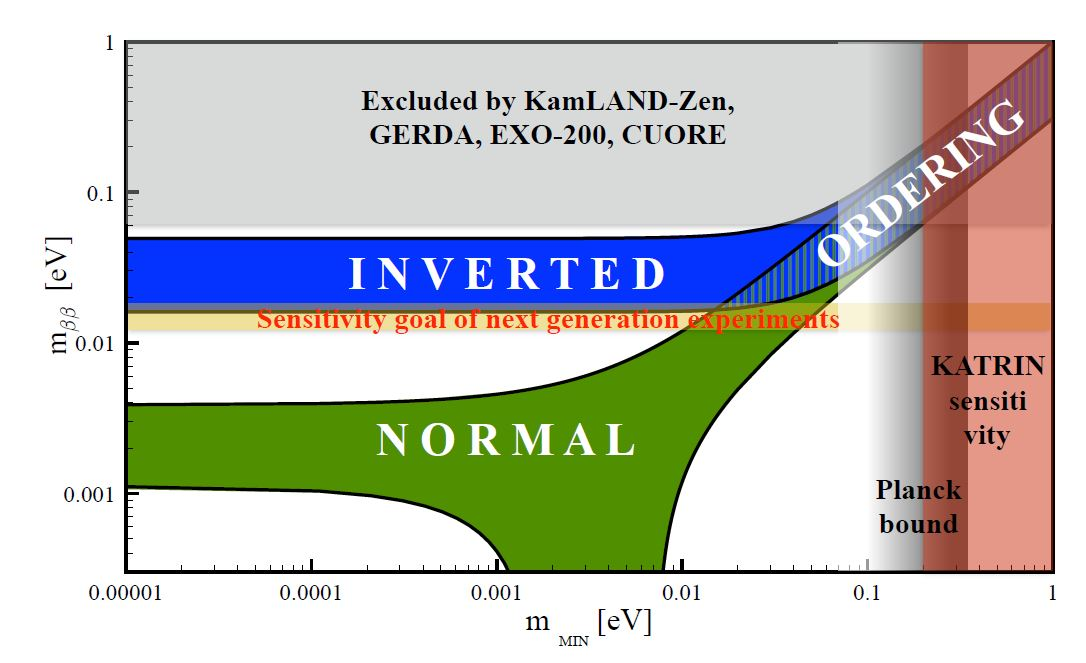
\includegraphics[scale=0.75]{doublebeta.jpg}
  \caption{The dependence of the effective Majorana mass $\abs{m_{\beta\beta}}$ on the minimum neutrino mass $m_{\mathrm{MIN}}$. From \cite{giuliani2020double}.}
  \label{fig:doublebeta}
\end{figure}


The upcoming generation of $\ndbd$ experiments seek to probe the entire range of $m_{\beta\beta}$ values allowed by the inverted hierarchy. Therefore, \emph{if it is established that the mass ordering is inverted,} then a null result from these $\ndbd$ experiments would demonstrate conclusively that \emph{the neutrino is not a Majorana particle.} Meanwhile, if the normal hierarchy is confirmed, then it becomes impossible to disprove the Majorana nature of the neutrino, since it may be hiding beneath a very small value of $m_{\beta\beta}$. (Of course, proving, as opposed to disproving, the Majorana nature remains possible via observation of $\ndbd$.) The mass hierarchy thus is extremely relevant to the task of determining the nature of neutrino mass, and, in turn, the large value of $\theta_{13}$ makes it possible to determine the MH via oscillation experiments. As shown by \autoref{eq:majoranaEffMass}, $\theta_{13}$ also plays an important role in the relation between $m_{\beta\beta}$ and the physical masses $m_i$.

Furthermore, as was mentioned earlier, the determination of the mass hierarchy would carry significant implications for the measurement of $\dcp$. Many experiments in the pipeline, particularly those that take advantage of matter effects, suffer from a degeneracy between $\dcp$ and the mass hierarchy, forcing them to quote two, possibly very different, confidence intervals for $\dcp$. The result is a considerably reduced overall sensitivity to leptonic CP violation. Knowledge of the hierarchy would eliminate this issue. With the knowledge that $\theta_{13}$ is large, measuring the mass hierarchy is an easier prospect in general, but in particular it allows for experiments, such as JUNO, that aim to efficiently determine the MH independently of $\dcp$. This acclerates the timeframe of MH determination, while also providing improved sensitivty to long-term $\dcp$(+MH) experiments such as DUNE and Hyper-Kamiokande. $\theta_{13}$, via its connection to the mass hierarchy, thus also provides an indirect boost to the $\dcp$ measurement effort, in addition to its direct influence on the oscillation probability.


\end{document}